\appendix
\appendixpage

The appendix contains all mathematical models relevant to the modelling of the component and system parameters of the payload designer.

\section{System Model}

\begin{table}[H]
\centering
\caption{System parameters.}
\label{tab:system-params}
\begin{threeparttable}
\begin{tabular}{@{}llllll@{}}
\toprule
Parameter             & Symbol            & Min & Typical & Max & Unit               \\ \midrule
Optical transmittance\tnote{1} & {$\eta_{optics}$} & 0   & -       & 1   & -                  \\
System mass           & {$M_{sys}$}       & 0   & -       & 200 & {\si{\gram}}       \\
System volume envelope   & {$\mathbf{V}_{sys}$}             & 0, 0, 0 & - & 100, 100, 200 & {\si{\milli\meter}}                                         \\
System wavelength\tnote{2}     & {$\lambda_{sys}$} & 0   & -       & -   & {\si{\nano\meter}} \\
Target spectral radiance\tnote{3} & {$L_{target}(\lambda)$} & 0       & - & -             & {\si{\watt\per\steradian\per\meter\squared\per\nano\meter}} \\ \bottomrule
\end{tabular}
\begin{tablenotes}
\item[1] A.k.a optical efficiency, transmittance ratio.
\item[2] Wavelength(s) of interest entering the optical system.
\item[3] Radiance reaching the satellite from the ground target as a function of wavelength. Data for this parameter is obtained through MODTRAN.
\end{tablenotes}
\end{threeparttable}
\end{table}


\subsection{Optical Transmittance} Y

\begin{equation}
    \eta_{optics} = \prod_{c \in C} c_{\eta}
\end{equation}

Where $\eta_{optics}$ is the net transmittance for the optical system, $c$ is an individual component in the system, $C$ is the set of all components in the system, and $c_{\eta}$ is the optical transmittance of an individual component.

\subsection{System Mass} Y

\begin{equation}
    M_{sys} = \sum_{c \in C} c_M
\end{equation}

Where $M_{sys}$ is the net mass of the system, $c$ is an individual component in the system, $C$ is the set of all components in the system, and $c_{M}$ is the mass of an individual component.

\subsection{System Volume Envelope} Y - merge

\begin{equation}
\bf{V} = \begin{bmatrix} V_x\\ V_y\\ V_z \end{bmatrix} = \begin{bmatrix} \max_{c \in C} c_{V_x}\\ \max_{c \in C} c_{V_y}\\ \sum_{c \in C} c_{V_z} \end{bmatrix}
\end{equation}

Where $V_x$, $V_y$, $V_z$ are the components of volume in the $x$, $y$, $z$ axes of the cubesat reference frame. See figure \ref{fig:cubesat-frame}. Assumes in-line design.

\section{Foreoptics Model} \todo{Jennifer}
The fore-optics of the spectrometer is the entrance optics, which serves as a telescope. Although its components are unknown, it can be treated as a black box.

\begin{figure}[H]
\centering
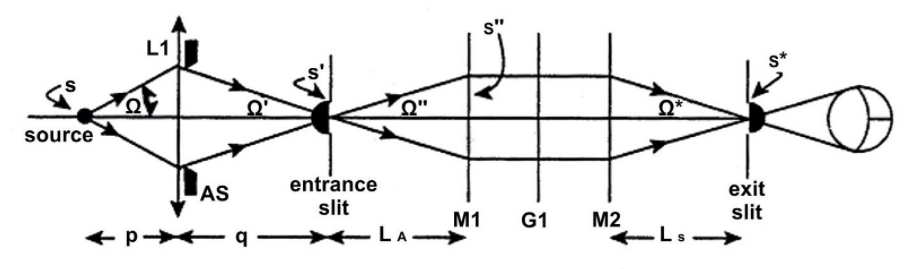
\includegraphics[width=1\textwidth]{figures/monochromator.PNG}
\caption{A monochromator system. \cite{Horiba_throughput_etendue}}
\label{fig:monochromator}
\end{figure}

$S$ = area of source\\
$S'$ = area of entrance slit\\
$S"$ = area of mirror M1\\
$S*$ = area of exit slit\\
$\Omega$ = half angle of light collected by L1\\
$\Omega'$ = half angle of light submitted by L1\\
$\Omega"$ = half angle of light collected by M1\\
$\Omega*$ = half angle of light submitted by M2\\
$L1$ = lens used to collect light from source\\
$M1$ = spherical collimating Czerny-Turner mirror\\
$M2$ = spherical focusing Czerny-Turner mirror\\
$AS$ = aperture stop\\
$LS$ = illuminated area of lens L1\\
$p$ = distance from object to lens L1\\
$q$ = distance from lens L1 to image of object at the entrance slit\\
$G1$ = diffraction grating


\begin{table}[H]
\centering
\caption{Foreoptic component parameters.}
\label{tab:foreoptic-params}
\begin{tabular}{@{}llllll@{}}
\toprule
Parameter                                              & Symbol              & Min & Expected & Max & Unit            \\ \midrule
Aperture diameter\tablefootnote{A.k.a aperture size.}       & {$d_{aperture}$}    &     &          &     & {\si{\mm}}      \\
Back focal length\tablefootnote{A.k.a back focal distance.} & {$\text{BFL}$}      &     &          &     & {\si{\mm}}      \\
Effective focal length                                 & {$\text{EFL}$}      &     &          &     & {\si{\mm}}      \\
F-number                                               & {$N$}               &     &          &     & -               \\
Image diameter\tablefootnote{A.k.a image diagonal.}         & {$d_{image}$}       &     &          &     & {\si{\mm}}      \\
Mass                                                   & {$m$}               &     & 80       &     & {\si{\g}}       \\
Maximum angle of incidence                             & {$\theta_{in,max}$} &     &          &     & {\si{\degree}}  \\
Mechanical length                                      & {$L$}               & 0   &          & 100 & {\si{\mm}}      \\
Numerical aperture                                     & {$\text{NA}$}       &     &          &     &                 \\
Spectral transmittance                                & {$T(\lambda)$}      & 0   & -        & 100 & {\si{\percent}} \\ \bottomrule
\end{tabular}
\end{table}

\subsection{Aperture Diameter} - Y
The aperture diameter of the foreoptics can be calculated by rearranging equation \ref{eq:f-num}:

\begin{equation}
    d=\frac{q}{f/value}=2q\times NA
\end{equation}

Where $NA$ is the numerical aperture, $q$ is the image distance from the fore-optic lens, $f/value$ is the f/number of the fore-optic system. When the object distance is very far (approaches infinity), the image distance is effectively the same as the focal length of the lens.

\subsection{Effective Focal Length} - Y
Effective Focal Length (EFL) is the distance from a principal plane of an optical lens to its imaging plane. The principle plane is a hypothetical plane where incident light rays can be considered to bend due to refraction, and the imaging plane is where the image is formed\cite{Edmund_lens_geometries}.\\
EFL is calculated using the thin lens equation \ref{eq:thin-lens}, as the image distance.

\subsection{Telecentricity} - Y \todo{Need to figure out exactly what Tymen meant->how this relates to us}
A telecentric lens is a lens whose chief rays are collimated. 

\begin{figure}[H]
\centering
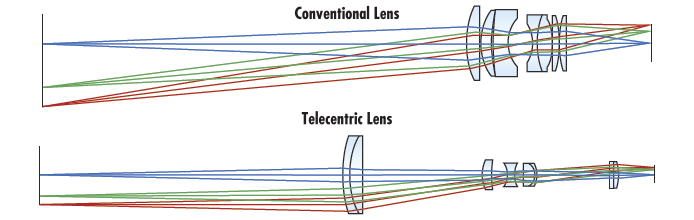
\includegraphics[width=0.75\textwidth]{figures/conventional-vs-telecentric-lens.png}
\caption{Conventional versus telecentric lens \cite{noauthor_undated-du}.}
\label{fig:conventional-vs-telecentric-lens}
\end{figure}


Chief rays are defined to be the rays from an off-axis point in the object passing through the center of the aperture stop for all points across the object (see figure \ref{fig:marginal-and-chief-rays})

\begin{figure}[H]
\centering
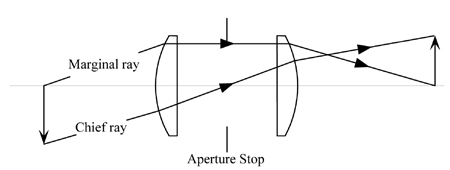
\includegraphics[width=0.5\textwidth]{figures/marginal-and-chief-rays.png}
\caption{Marginal and chief rays \cite{noauthor_undated-cw}}
\label{fig:marginal-and-chief-rays}
\end{figure}
 
The primary benefit of telecentricity is that the system magnification is insensitive to slight changes in image distance. In other words, a telecentric lens produces an orthographic view of the scene it is pointed at, as opposed to a perspective view\footnote{Think back to elementary school art class.}. Telecentricity is very important in our system because it has to be matched\todo{Tymen's explanation is ambiguous. How is it matched?} to our relay / diffraction stage optics, otherwise we may end up with severe vignetting (Tymen Nagel from Chromar Technologies).

A telecentric lens may be characterized by its degree of telecentricity, or simply telecentricity, which is the deviation of the principal ray from parallelism to the optical axis \cite{Sischka2015-jc}. Telecentricity is typically measured in degrees. So, for example, a lens with an object-space telecentricity of \SI{0.3}{\degree} will accept light at angles of up to \SI{0.3}{\degree} away from parallel to the optical axis \cite{Sischka2015-jc}. In practice, no telecentric lens is perfect. That is, no telecentric lens images only light entering parallel to the optical axis \cite{Sischka2015-jc}.

The field of view of an object-space telecentric lens cannot exceed the size of the objective lens; so it cannot be used to image anything larger than the objective. This means that they are generally larger than an equivalent fixed focal length lens, which is a direct consequence of the fact that they have no angular field of view \cite{Sischka2015-jc}. If a lens is not telecentric, it is either entocentric or hypercentric \cite{Wikipedia_contributors_undated-tx}. Common lenses are usually entocentric.


\subsection{Magnification} - Y

The magnification of the fore-optics is calculated by \cite{Horiba_entrance_optics}:

\begin{equation}
    M = \frac{q}{p}
\end{equation}

Where $M$ is the magnification, $q$ is the image distance from the fore-optic lens, $p$ is the object distance from the fore-optic lens, as seen in Figure \ref{fig:monochromator}.

\subsection{Numerical Aperture} - Y
Numerical Aperture is the light gathering power of an optic, characterizing the range of angles of light rays that can enter or exit an optical component (e.g. lens, slit) \cite{Horiba_monochromator}.

\begin{equation}
    NA = \mu\sin\Omega
\end{equation}

Where $\mu$ is the refractive index (1 in air), $\Omega$ is the angle of the marginal ray from the optical axis (from Figure \ref{fig:monochromator}).

``The numerical aperture (1/f-number/2) sets the angle of the rays at the edge of the focused cone of energy. This must be tied in with the maximum AOI at the edge of the field (acceptable deviation from perfect telecentricity). This should be considered when determining the first order specifications." ---Tymen Nagel from Chromar Technologies

\subsection{Back Focal Length} - Y
Back focal length (BFL) is defined as the distance from the backmost mechanical plane of the fore-optics to the focal plane, where the slit is mounted. This is thus a purely mechanical constraint, and consultation with the Payload Structures team is warranted. The \texttt{program} will not include BFL as an optical parameter.

\subsection{F/value (f/number)} - Y
The F value, often known as the f/number, of a lens system is the ratio of the image distance to the diameter of the slit:

\begin{equation} \label{eq:f-num}
    f/value = \frac{1}{2NA} = \frac{q}{d}
\end{equation}

Where $NA$ is the numerical aperture, $q$ is the image distance from the fore-optic lens, $d$ is the diameter of the aperture in the fore-optic system. When the object distance is very far (approaches infinity), the image distance is effectively the same as the focal length of the lens.\\
Note: $NA = sin(\Omega)$, from Figure \ref{fig:monochromator}, which approximates to $\frac{1}{2f/number}$ \cite{Horiba_monochromator}.

The f/number is usually set by adjusting the diaphragm/aperture in most lens systems. The lower the lens’ f/number, the larger the iris, and more light is able to pass through the system (greater throughput). The f/number usually increases by multiple of $\sqrt{2}$, since the aperture area typically varies by a factor of 2 \cite{Hollows_undated}.

\subsection{Geometric Etendue} - Y
The geometric etendue of an optical system is its ability to accept light, characterized by the maximum beam size the optical component can accept. As such, it can limit light throughput of the spectrometer. It is calculated by \cite{Horiba_throughput_etendue}:

\begin{equation}
    d^2G = \frac{dS}{dQ}
\end{equation}

\begin{equation}
    G = \iint\frac{dS}{dQ}
\end{equation}

Where $G$ is the geometric etendue, $S$ is the area of the emitting source, $Q$ is the solid angle into which light propagates (2$\Omega$ in Figure \ref{fig:monochromator}).
Through integration:

\begin{equation}
    G = \pi\Sigma\sin^2\Omega
\end{equation}

Where $G$ is the geometric etendue, $\Omega$ is the angle of the marginal ray from the optical axis.
In order to optimize throughput, the maximum beam size that is acceptable by the optical component should be used, and:

\begin{equation}
    G = \pi S\sin^2\Omega = \pi S'\sin^2\Omega' = \pi S"\sin^2\Omega" = \pi S^*\sin^2\Omega^*
\end{equation}

\subsection{Flux} - Y
From the geometric etendue, flux, defined as “energy/time (photons/sec, or watts) emitted from a light source or slit of given area, into a solid angle at a given wavelength (or bandpass)”, can be calculated \cite{Horiba_throughput_etendue}:

\begin{equation}
    \phi = B\times G
\end{equation}

\begin{equation}
    \phi = B\pi S'\sin^2\Omega'
\end{equation}

Where $B$ is the radiance of the source, $S'$ is the area of the entrance slit or emitting source, $\Omega'$ is the angle of the marginal ray from the optical axis; shown in Figure \ref{fig:monochromator}.

\section{Slit Model} \todo{Jennifer}

\begin{figure}[H]
\centering
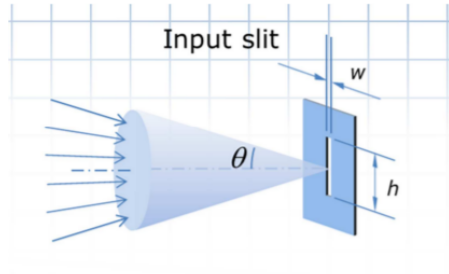
\includegraphics[width=0.6\textwidth]{figures/entrance slit.PNG}
\caption{Light arriving at the entrance slit of a spectrometer. \cite{Ibsen_photonics_coupling}}
\label{fig:entrance-slit}
\end{figure}

The light output from the fore-optics passes through a narrow slit, which plays a large role in determining the throughput of the optical system (i.e. amount of light, measured by photon flux) and resolution. These are affected by the size (length and width) of the entrance slit; slit length in the horizontal direction and slit width in the vertical. In figure \ref{fig:entrance-slit}, which shows the slit sideways, $h$ is the length and $w$ is the width. The standard slit length is 1 mm, with options of up to 2 mm available as well \cite{B&W_Tek}; since the spectrometer should have a magnification of 1, the slit length should equal the detector width. Slit widths range from 5$\mu m$ to 800$\mu m$, with standard sizes: 10, 14, 25, 50, 100 and 200 $\mu m$ \cite{StellarNet}. It must be placed exactly within the optical path of the spectrometer, its distance from the fore-optics dependent on the image distance from the fore-optic lens \cite{Horiba_entrance_optics}, and distance from the collimator dependent on the focal point of the collimation lens \cite{Ibsen_photonics_design}.\\

Decreasing the slit width blocks incoming light travelling at larger angles, with respect to the optical axis, improving resolution while decreasing light throughput. Therefore, both factors must be taken into consideration when optimizing slit width \cite{Optecks}.

\subsection{Field of View} - merge
The field of view (FOV), or angular field of view (AFOV), is the full angle (degrees) from the fore-optic lens outwards, and has a horizontal and vertical measurement \cite{Edmund_fov}.\\
In the horizontal direction:

\begin{equation}
    FOV_h = 2\times\arctan\frac{x_h}{2f}
\end{equation}

Where $x_h$ is the slit length (horizontal direction) and $f$ is the focal length of the fore-optics.\\
In the vertical direction:

\begin{equation}
    FOV_v = 2\times\arctan\frac{x_v}{2f}
\end{equation}

Where $x_v$ is the slit width (vertical direction) and $f$ is the focal length of the fore-optics.\\
From the FOV, we can calculate the instantaneous field of view (IFOV) in both directions, the angle subtended by the geometrical projection of single detector element to the target surface \cite{Specim}.\\
Because the spectrometer has a magnification of $1$, the IFOV in the horizontal direction is:

\begin{equation}
    IFOV_h = \frac{FOV_h}{n}
\end{equation}

Where $FOV_h$ is the horizontal FOV and $n$ is the number of pixels on the detector in the horizontal direction.\\
For the vertical iFOV, if the detector's pixel pitch is smaller than the slit width:

\begin{equation}
    IFOV_v = 2\times\arctan\frac{s}{2f}
\end{equation}

Where $s$ is the pixel size and $f$ is the focal length of the fore-optics,

\subsection{Image Width} - pending
The image width of the entrance slit is estimated as \cite{B&W_Tek}:

\begin{equation}
    W_i = \sqrt{M^2\times W_s^2 + W_o^2}
\end{equation}

Where $M$ is the magnification of the optical bench (i.e. ratio of the focal length of the focusing lens to that of the collimating lens), $W_s$ is entrance slit width, and $W_o$ is object width (in this case, the image broadening from the optical bench).

\subsection{Slit Width}

\begin{figure}[H]
\centering
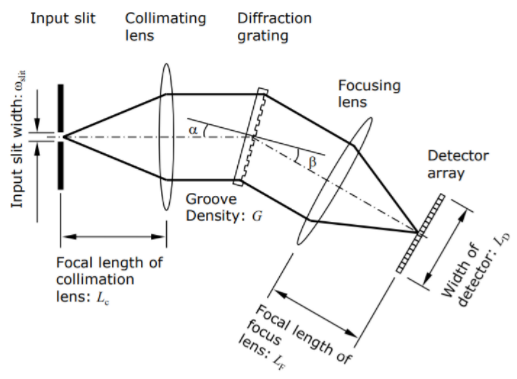
\includegraphics[width=0.7\textwidth]{figures/spectrometer design.PNG}
\caption{A typical set-up of a spectrometer. \cite{Ibsen_photonics_design}}
\label{fig:spectrometer-design}
\end{figure}

It is suggested to select a slit width after other components have already been selected, since:

\begin{equation}
    w_{slit} = \frac{L_D}{M}
\end{equation}

Where $L_D$ is the detector width, $M$ is the spectrometer magnification, seen in Figure \ref{fig:spectrometer-design}.\\
Since $M$ should be as close to 1 as possible, this provides the maximum value of the slit length, to project across the whole width of the detector.\\
Assumptions: the spectrometer geometry is either transmission grating based (LGL, which stands for "lens-grating-lens") or crossed Czerny-Turner.

\section{Lens Models}
The lens models we derive here apply for lenses operating on light which is collimated\footnote{\href{https://en.wikipedia.org/wiki/Collimated_beam}{Collimated light} is light whose rays propagate in parallel.} either on the onset or outset. We focus on these two scenarios because the payload specifically makes use of lenses acting as either \textit{collimators} or \textit{focusers}. A collimator takes a point source of light (i.e. light exiting the slit) and produces a collimated beam. A focuser takes collimated light and produces an image (i.e. the lens responsible for focusing the diffracted light from the diffractor onto the sensor). Despite being a distinguishing factor between candidate models, chromatic aberrations are not taken into account for the reasons noted in section \ref{sec:scope}.


\subsection{Thin Singlet Lens Model} - Y \label{sec:thin-singlet-model}

A thin lens is a mathematical approximation of a real lens. For sufficiently thin lenses, the thin lens equations are an adequate description of the characteristics of the lens \cite{Boundless_undated-to}.

The following assumptions are made for all the defining equations:

\begin{itemize}
    \item Rays are paraxial.\footnote{Paraxial rays are rays of light at small enough angles from the optical axis that they are well described by the small angle approximation \cite{noauthor_undated-wt}.} 
    
    \item Lens is of negligible thickness.
    
    \item Incoming light to the focuser or outgoing light from the collimator is perfectly collimated.
    
    \item Does not account for field curvature.\footnote{\href{https://en.wikipedia.org/wiki/Petzval_field_curvature}{Field curvature} is a type of optical aberrations in which a flat object normal to the optical axis cannot be brought properly into focus on a flat image plane, but instead the focal plane ends up curved.}
\end{itemize}


\begin{figure}[H]
    \centering
    \subfloat[\centering Collimator]{{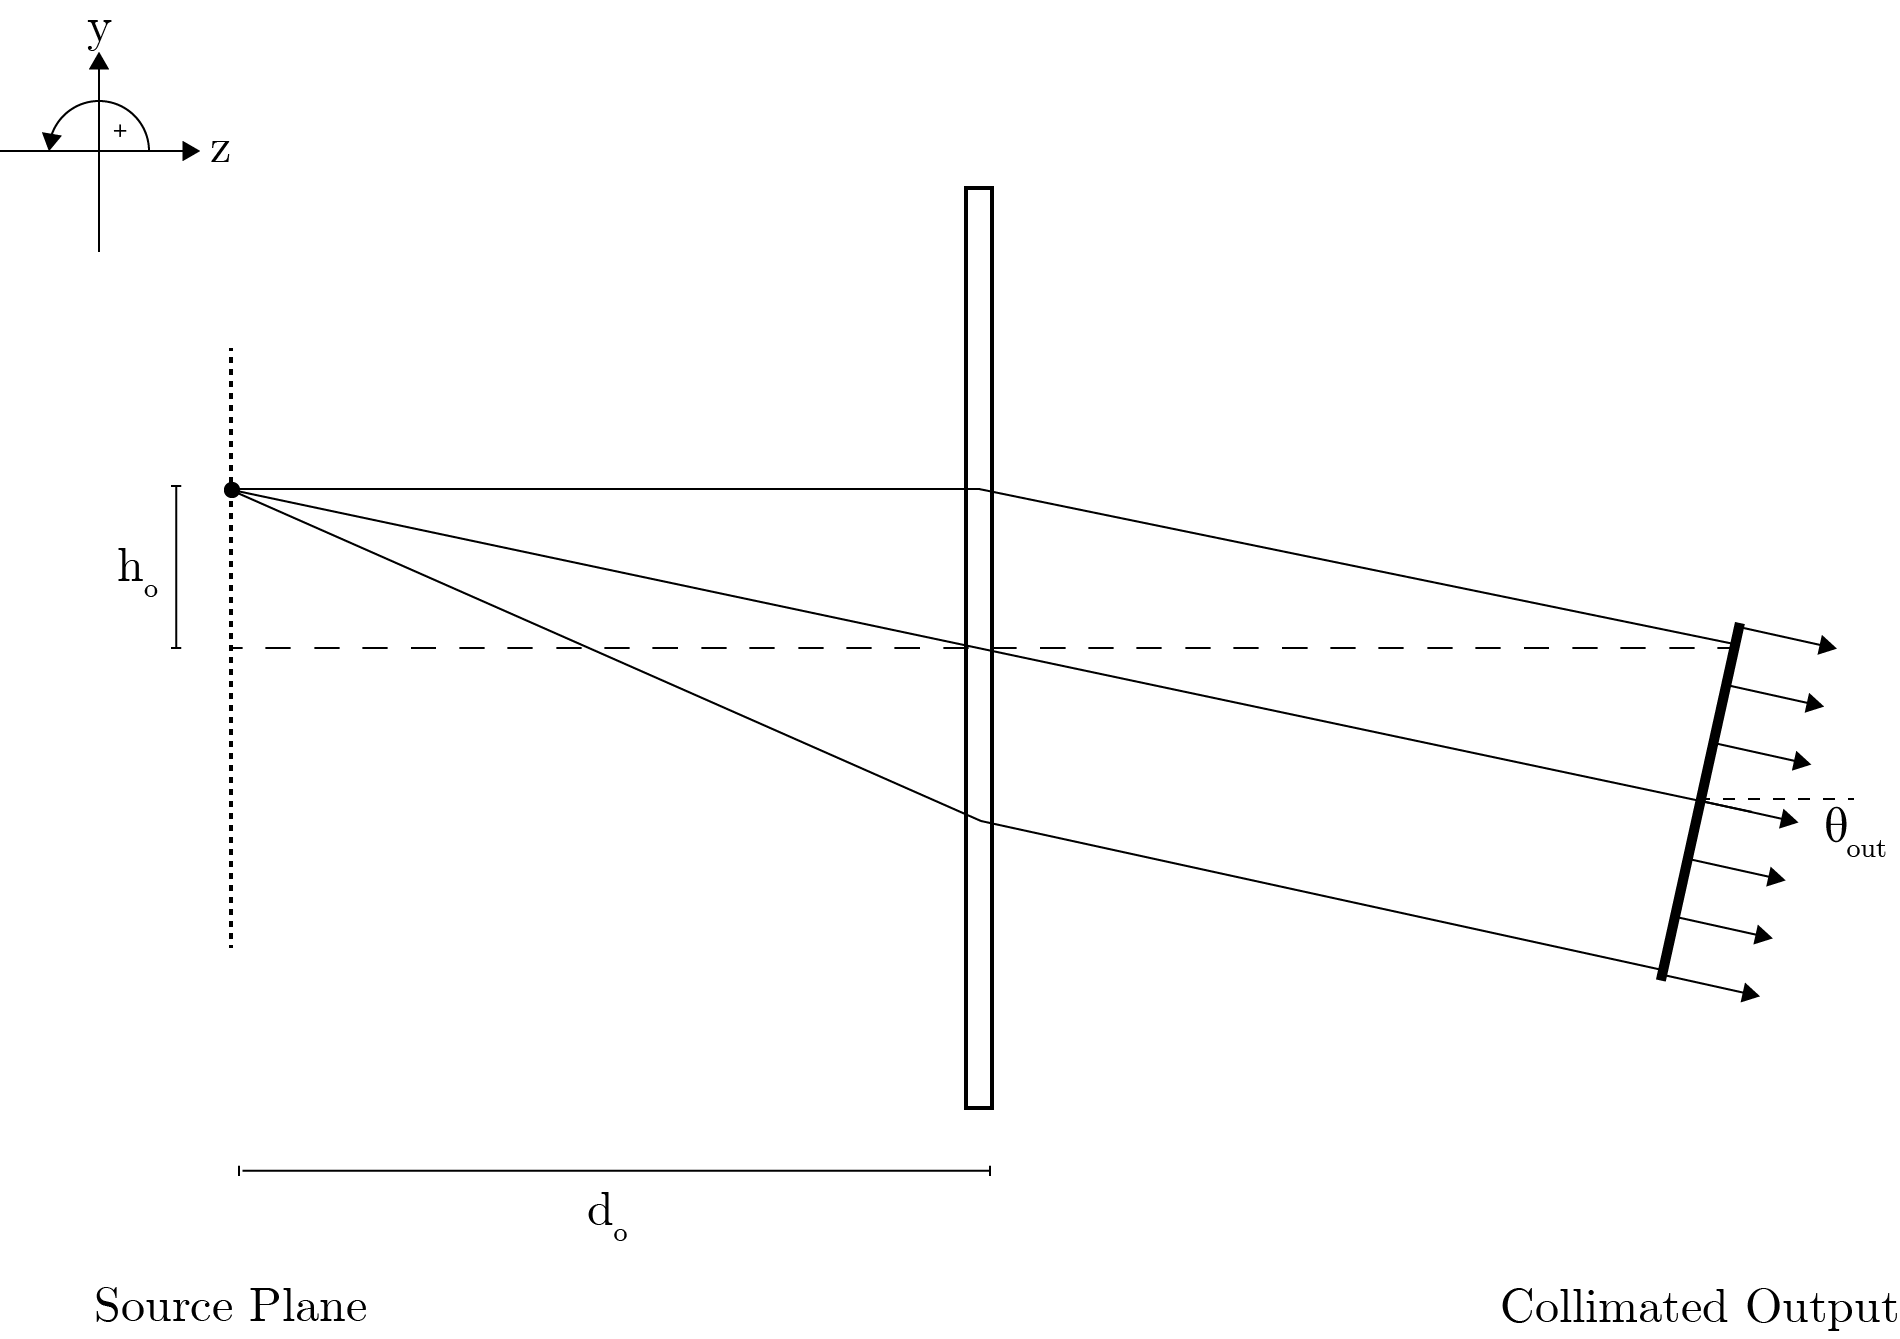
\includegraphics[width=0.45\textwidth]{figures/thin-collimator-model.png}}}
    \qquad
    \subfloat[\centering Focuser]{{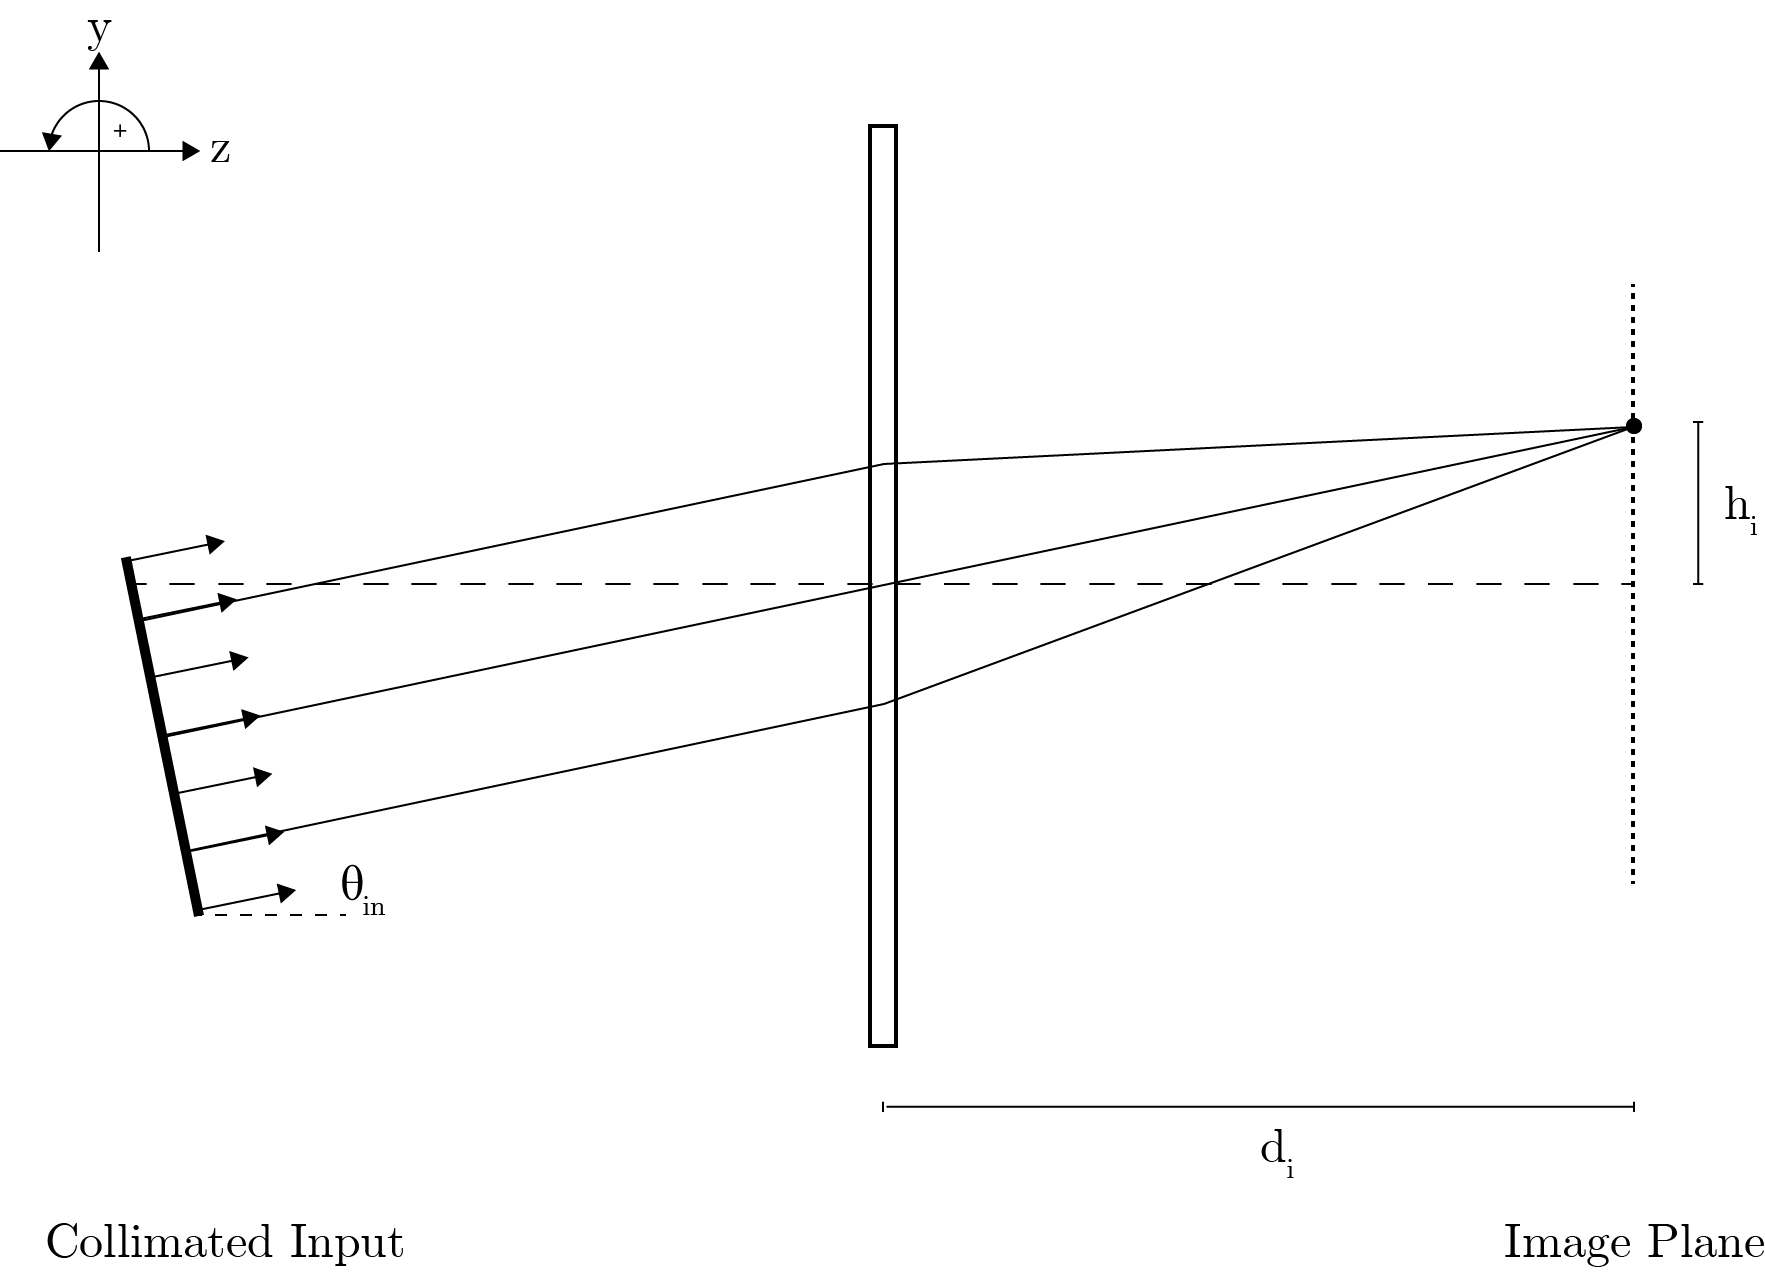
\includegraphics[width=0.45\textwidth]{figures/thin-focuser-model.png}}}  
    \caption{Thin singlet models.}
    \label{fig:thin-singlet-lens-models}
\end{figure}

\begin{table}[H]
\centering
\caption{Thin lens model parameters.}
\label{tab:thin-lens-parameters}
\begin{tabular}{@{}llllll@{}}
\toprule
Parameter                 & Symbol           & Min  & Typical & Max & Unit           \\ \midrule
Diameter                  & {$D$}            & 0    & -       & -   & {\si{\mm}}     \\
Focal length              & {$f$}            & -    & -       & -   & {\si{\mm}}     \\
Image height              & {$h_i$}          & -    & -       & -   & {\si{\mm}}     \\
Image plane distance      & {$d_i$}          & 0    & -       & -   & {\si{\mm}}     \\
Incoming collimated angle & {$\theta_{int}$} & -180 & 0       & 180 & {\si{\degree}} \\
Mass                      & {$M$}            & 0    & -       & -   & {\si{\g}}      \\
Source height             & {$h_o$}          & -    & -       & -   & {\si{\mm}}     \\
Source plane distance     & {$d_o$}          & 0    & -       & -   & {\si{\mm}}     \\
Outgoing collimated angle & {$\theta_{out}$} & -180 & 0       & 180 & {\si{\degree}} \\
Transmittance             & {$T(\lambda)$}   & 0    & -       & 1   & -              \\ \bottomrule
\end{tabular}
\end{table}


\subsubsection{Source \& Image Distances} - Y \label{sec:thin-object-image-distances}
The source distance of a thin lens is the distance between a point source of light and the lens. The image distance is the distance between the lens and the image plane. This distance is approximated by the thin lens equation \cite{noauthor_undated-zn}:

\begin{equation} \label{eq:thin-lens}
    \frac{1}{f} = \frac{1}{d_o} + \frac{1}{d_i}
\end{equation}

Where $f$ is the focal length of the thin lens, $d_o$ is the distance from the source to the lens, and $d_i$ is the distance from the lens to the image.

\begin{enumerate}[(a)]
    \item In the case of a thin focuser, input rays are parallel, and may be represented by a source that is an infinite distance away. Output rays converge, hence the image is at a finite distance after the lens. Thus:
    \begin{equation}
        \frac{1}{f} = \lim_{d_o\to\infty} \frac{1}{d_o} + \frac{1}{d_i} = \frac{1}{d_i}
    \end{equation}
    
    \begin{equation} \label{eq:image-distance}
        \Rightarrow \ \boxed{d_i = f}    
    \end{equation}
    
    \item In the case of a thin collimator, incoming rays diverge, hence the source is at a finite distance before the lens. Outgoing rays are collimated, which may be represented by an image at an infinite distance away. Thus:
    \begin{equation}
        \frac{1}{f} = \lim_{d_i\to\infty} \frac{1}{d_o} + \frac{1}{d_i} = \frac{1}{d_o}
    \end{equation}
    
    \begin{equation} \label{eq:source-distance}
        \Rightarrow \ \boxed{d_o = f}
    \end{equation}
\end{enumerate}

\subsubsection{Source \& Image Heights} 
Source and image heights are measured perpendicularly from the optical axis to the outermost point of the source/image.

For a thin focuser, since the source distance is effectively infinity, it is not sensible to think of a source height. The image height is the perpendicular distance measured from the optical axis to the outermost point on the focal plane where incoming collimated light converges.

For a thin collimator, the source height is the perpendicular distance measured from the optical axis to the outermost point of the source. Conversely, since the image distance is effectively infinity, the concept of image height does not hold.

\begin{enumerate}[(a)]
    \item A parallel bundle of rays incident on a focuser will focus at the intersection of the centre ray with the focal plane \cite{Boundless_undated-to, N_W_Edmund1968-fm}. In the paraxial regime:

    \begin{align}
    \tan\left( \theta_{in} \right) \simeq \theta_{in} &= \frac{h_i}{d_i} \\
    h_i &= d_i \theta_{in}
    \end{align}
    Where $h_i$ is the height of the point of focus for the ray bundle on the focal plane from the optical axis, $d_i$ is the distance of the focal plane from the lens, and $\theta_{in}$ is the incoming angle of the collimated rays.
    
    We know from section \ref{sec:thin-object-image-distances} that for a thin lens, the focal length defines the distance from the lens to the focal plane ($d_i = f$). Thus,
    
    \begin{equation} \label{eq:image-height}
        \boxed{h_i = f \theta_{in}}
    \end{equation}
    
    \item Similarly, the source height for a collimator can be found as:

    \begin{align}
    \tan\left(\theta_{out} \right) \simeq \theta_{out} &= -\frac{h_o}{d_o} \\
    h_o &= -d_o \theta_{out}
    \end{align}
    
    \begin{equation} \label{eq:source-height}
        \boxed{h_o = -f \theta_{out}}
    \end{equation}
\end{enumerate}

\subsubsection{Focal Length}
We can derive the focal length for the thin lens in two ways:

\begin{enumerate}[(a)]
    \item For a thin focuser:
    \begin{enumerate}[(i)]
        \item From image distance. Rearranging \eqref{eq:image-distance}:
    
        \begin{equation}
            \boxed{f = d_i}
        \end{equation}
        
        \item From image height and incoming angle. Rearranging \eqref{eq:image-height}:
    
        \begin{equation}
            \boxed{f = \frac{h_i}{\theta_{in}}}
        \end{equation}
    \end{enumerate}
    
    \item For a thin collimator:
    \begin{enumerate}[(i)]
        \item From source distance. Rearranging \eqref{eq:source-distance}:
        
        \begin{equation}
            \boxed{f = d_o}
        \end{equation}
        
        \item From source height and outgoing angle. Rearranging \eqref{eq:source-height}:
        
        \begin{equation}
            \boxed{f = -\frac{h_o}{\theta_{out}}}
        \end{equation}
    \end{enumerate}
\end{enumerate}


\subsubsection{Magnification} \label{sec:thin-magnification} \todo{explain when mag of zero occurs for snr section}
The concept of magnification for collimated light does not apply, as linear magnification is undefined. To see why, we begin with the definition of linear magnification  \cite{Boundless_undated-to}:

\begin{equation}
    m = \frac{h_i}{h_o} = - \frac{d_i}{d_o}
\end{equation}

Where $m$ is the linear magnification, $h_i$ is the image height, $h_o$ is the object height, $d_i$ is the image distance from the lens, and $d_o$ is the object distance from the lens. Taking the limit as $d_i$ or $d_o$ go to infinity yields an undetermined magnification.

\subsection{Thick Singlet Model} \todo{Stephanie}
\label{sec:thick-singlet-model}

A thick lens is a lens whose thickness is not negligible. Therefore, we have to consider the refraction of a light ray at both surfaces of the thick lens which are a distance apart (i.e., the image formed by the first surface is treated as the object for the second surface).

\begin{figure}[H]
\centering
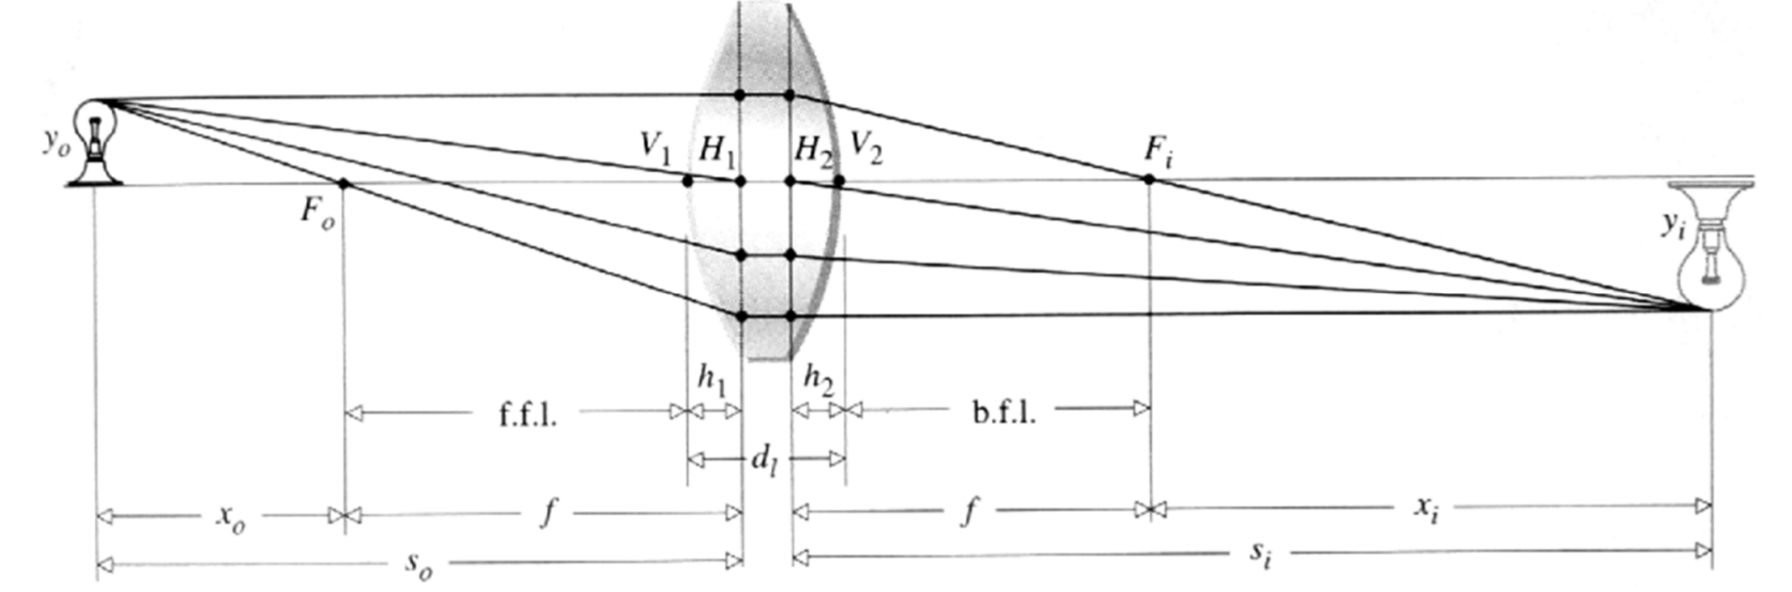
\includegraphics[width=1\textwidth]{figures/thick-lens.png}
\caption{The thick lens model \cite{Jones2013}.}
\label{fig:thick-lens-model}
\end{figure}

\subsubsection{Position of the Principal Planes}

To compute the position of the image of an object at a given distance from the thick lens, we need to calculate the position of the principal planes of the thick lens. All refraction is considered to occur at the principal planes, and for a given lens, the principal planes do not depend on object position \cite{Nave2017}.

For a bispherical lens:

\begin{itemize}
    \item Position of the first (or primary) principal plane, $H_1$ \cite{Nave2017}:
\end{itemize}

\begin{equation} \label{eq:thick-first-principal-plane}
    h_1 = -\frac{f(n-1)d}{R_2 n}
\end{equation}

\begin{itemize}
    \item Position of the second (or secondary) principal plane, $H_2$ \cite{Nave2017}:
\end{itemize}

\begin{equation} \label{eq:thick-second-principal-plane}
    h_2 = -\frac{f(n-1)d}{R_1 n}
\end{equation}

Where $h_1$ and $h_2$ are the distances between the vertices of the lens and the principal planes, $f$ is the focal length of the lens, $n$ is the index of refraction of the lens, and $d$ is the thickness of the lens (i.e., the distance between the two vertices of the lens).

$R_1$ and $R_2$ are the radii of curvature of the thick lens. If the vertex of the lens surface lies in front of the centre of curvature of that surface, the radius of curvature is positive. If the vertex lies behind the centre of curvature, the radius of curvature is negative \cite{Serbanescu2013}. (E.g. in Figure \ref{fig:thick-lens-model}, the front (left) surface has positive radius of curvature while the back (right) surface has negative.)

These equations assume that the light rays are close to the optical axis (i.e., in the paraxial region). Away from the paraxial region, the principal planes bend as spheres instead \cite{noauthor-2021}.

\subsubsection{Equivalent Focal Length}

% For a thick lens in a medium \cite{}:

% \begin{equation}
    % \frac{1}{f} = \frac{n_l-n_m}{n_m}\left(\frac{1}{R_1}-\frac{1}{R_2}+\frac{n_l-n_m}{n_m}\cdot\frac{d}{n_lR_1R_2} \right) 
% \end{equation}

The Lensmaker's equation calculates the focal length of a thick lens in a vacuum \cite{Jones2013, Boundless_undated-to, Nave2017}:

\begin{equation}
    \frac{1}{f} = (n-1)\left( \frac{1}{R_1}-\frac{1}{R_2}+\frac{(n-1)d}{n R_1 R_2} \right)
\end{equation}

\hspace{8pt} Rearranging for $f$:

\begin{equation}
    f = \frac{n R_1 R_2}{(R_2-R_1)(n-1)n + (n_l-1)^2 d}
\end{equation}

% \hspace{8pt} Rearranging for $f$:

% \begin{align*} % derivation
%     \frac{1}{f} &= \frac{n_l-n_m}{n_m} \cdot \frac{n_l n_m (R_2 - R_1) + (n_l - n_m) d}{R_1 R_2 n_l n_m} \\
%     \frac{1}{f} &= \frac{n_l n_m (R_2 - R_1) (n_l - n_m) + (n_l - n_m)^2 d}{R_1 R_2 n_l n_m^2}
% \end{align*}

% \begin{equation}
    % f = \frac{n_m^2 n_l R_1 R_2}{(R_2 - R_1)(n_l - n_m) n_m n_l + (n_l - n_m)^2 d}
% \end{equation}

Where $f$ is the focal length of the lens, $n$ is the index of refraction of the lens, $d$ is the thickness of the lens (i.e., the distance between the two vertices of the lens), and $R_1$ and $R_2$ are the radii of curvature of the thick lens. 

Both equations assume that the medium on both sides of the lens have the same index of refraction. Therefore, the focal lengths from the two principal planes are equal \cite{Serbanescu2013}.

\subsubsection{Object and Image Distances from Principal Planes}

For a thick lens, we use the same equation as the thin lens to calculate image distance \cite{Jones2013}:

\begin{equation} \label{eq:thick-object-image-dists}
    \frac{1}{f} = \frac{1}{s_o} + \frac{1}{s_i}
\end{equation}

Where $f$ is the focal length of the thick lens, $s_o$ is the distance from the object to the first principal plane, and $s_i$ is the distance from the second principal plane to the image.

For a thick focuser, input rays are parallel, so the object is at an infinite distance from the lens. Output rays converge, so the image is at a finite distance from the lens. 

\begin{equation}
    \frac{1}{f} = \lim_{s_o\to\infty} \frac{1}{s_o} + \frac{1}{s_i} = \frac{1}{s_i}
\end{equation}
Thus:
\begin{equation}
    s_i = f
\end{equation}

For a thick collimator, incoming rays diverge, so the object is at a finite distance from the lens. Outgoing rays are collimated, so the image is at an infinite distance from the lens.

\begin{equation}
    \frac{1}{f} = \lim_{s_i\to\infty} \frac{1}{s_o} + \frac{1}{s_i} = \frac{1}{s_o}
\end{equation}
Thus:
\begin{equation}
    s_o = f
\end{equation}

\subsubsection{Source/Image Heights and Emergent/Incident Ray Angles}

The following equations make the assumption that the lens is in a vacuum (i.e. $n_m=1$).

\begin{figure}[H]
\centering
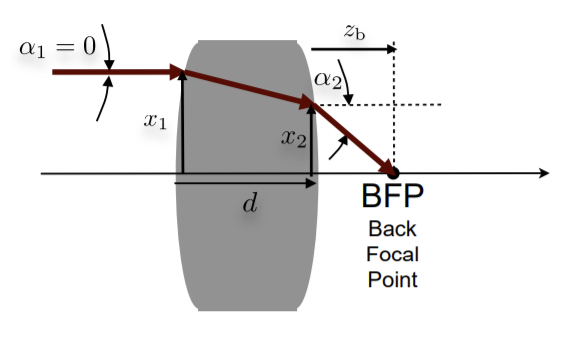
\includegraphics[width=0.5\textwidth]{figures/thick-lens-focuser.png}
\caption{The thick lens focuser model \cite{MIT_Lec5}.}
\label{fig:thick-lens-focuser-model}
\end{figure}

For a focuser lens, the image height ($x_2$) can be found through the following matrix approach, provided the paraxial approximation remains valid \cite{MIT_Lec4, MIT_Lec5}:
\[ 
\begin{bmatrix} a_2\\x_2 \end{bmatrix} =
\begin{bmatrix}
1 & 0\\
z_b & 1
\end{bmatrix}
\begin{bmatrix}
1 + \frac{n-1}{n} \frac{d}{R_2} & \frac{-1}{f}\\
\frac{d}{n} & 1 - \frac{n-1}{n} \frac{d}{R_1}
\end{bmatrix}
\begin{bmatrix}
a_1\\
x_1
\end{bmatrix}
\]

Where $a_1$ and $a_2$ are the angles of the incident and emergent rays relative to the optical axis, $x_1$ is the height of the incident beam at the lens surface, $x_2$ is the image height, $d$ is the thickness of the lens, $z_b$ is the back focal length, $f$ is the effective focal length, $n$ is the index of refraction of the lens, and $R_1$ and $R_2$ are the radii of curvature of the lens. 

After multiplying the first 2 matrices:
\[ 
\begin{bmatrix} a_2\\x_2 \end{bmatrix} =
\begin{bmatrix}
1 + \frac{n-1}{n}\frac{d}{R_2} & \frac{-1}{f}\\
z_b\left(1 + \frac{n-1}{n}\frac{d}{R_2}\right) + \frac{d}{n} & \frac{-z_b}{f} + 1 - \frac{n-1}{n}\frac{d}{R_1}
\end{bmatrix}
\begin{bmatrix}
a_1\\
x_1
\end{bmatrix}
\]

$z_b$, the back focal length, is equal to $f\left(1 - \frac{n-1}{n}\frac{d}{R_1}\right)$ \cite{MIT_Lec5}. Simplifying and solving for $x_2$:
\begin{equation}
    \boxed{x_2 = a_1f}
\end{equation}

\begin{figure}[H]
\centering
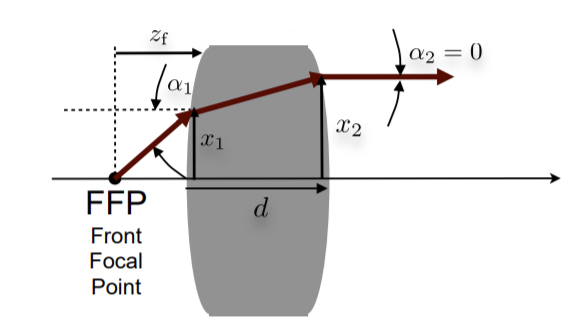
\includegraphics[width=0.5\textwidth]{figures/thick-lens-collimator.png}
\caption{The thick lens collimator model \cite{MIT_Lec5}.}
\label{fig:thick-lens-collimator-model}
\end{figure}

For a collimating lens, a similar approach with a rearrangement of matrices can be followed to calculate the angle of the emergent ray ($a_2$) from object height ($x_1$) \cite{MIT_Lec4, MIT_Lec5}:

\[ 
\begin{bmatrix} a_2\\x_2 \end{bmatrix} =
\begin{bmatrix}
1 + \frac{n-1}{n} \frac{d}{R_2} & \frac{-1}{f}\\
\frac{d}{n} & 1 - \frac{n-1}{n} \frac{d}{R_1}
\end{bmatrix}
\begin{bmatrix}
1 & 0\\
z_f & 1
\end{bmatrix}
\begin{bmatrix}
a_1\\
x_1
\end{bmatrix}
\]

Where $a_1$ and $a_2$ are the angles of the incident and emergent rays relative to the optical axis, $x_1$ is the object height, $x_2$ is the height of the emergent beam at the lens surface, $d$ is the thickness of the lens, $z_f$ is the front focal length, $f$ is the effective focal length, $n$ is the index of refraction of the lens, and $R_1$ and $R_2$ are the radii of curvature of the lens. 

After multiplying the first 2 matrices:
\[ 
\begin{bmatrix} a_2\\x_2 \end{bmatrix} =
\begin{bmatrix}
1 +\frac{n-1}{n}\frac{d}{R_2} - \frac{z_f}{f} & \frac{-1}{f}\\
z_f\left(1 - \frac{n-1}{n}\frac{d}{R_1}\right) + \frac{d}{n} & 1 - \frac{n-1}{n}\frac{d}{R_1}
\end{bmatrix}
\begin{bmatrix}
a_1\\
x_1
\end{bmatrix}
\]

$z_f$, the front focal length, is equal to $f\left(1 + \frac{n-1}{n}\frac{d}{R_2}\right)$ \cite{MIT_Lec5}. Simplifying and solving for $a_2$:
\begin{equation}
    \boxed{a_2 = \frac{-x_1}{f}}
\end{equation}

% \subsubsection{Image Distance from Focal Point}
% Commented this part out because this only works when d_i and d_o do not go to infinity. (Image/object is at focal point, so distance from focal point = 0)

% To calculate the image distance from the focal point \cite{Jones2013}:

% \begin{equation}
    % f^2 = x_o x_i
% \end{equation}

% Rearranging for $x_i$:

% \begin{equation}
    % x_i = \frac{f^2}{x_o}
% \end{equation}

% Where $f$ is the focal length of the thick lens, $x_o$ is the distance from the object to the first focal point, and $x_i$ is the distance from the second focal point to the image.

\subsubsection{Magnification}

Magnification of a thick lens can be calculated by \cite{Jones2013}:

\begin{equation}
    m_T = -\frac{s_i}{s_o} = \frac{h_i}{h_o}
\end{equation}

Where $m_T$ is the magnification of the lens, $s_o$ is the distance from the object to the first principal plane, $s_i$ is the distance from the second principal plane to the image, $h_o$ is the height of the object, and $h_i$ is the height of the image.

This equation cannot be used to calculate the object or image height in the case of a focuser or collimator because by taking the limit as $s_i$ or $s_o$ goes to infinity, the magnification is undefined. 

\subsection{Achromatic Doublet Model} - move parts into TDD for component selection \todo{Amy}

An achromatic doublet is composed of two elements: a concave lens (made of flint glass, which has a high refractive index) and a convex lens (made of crown glass, which has a low refractive index) \cite{EdmundOptics}.

Chromatic aberration is the effect caused by the difference in refractive index for a given material at different wavelengths. This can be reduced by an achromatic doublet as its two lenses compensate for their respective dispersions. Other types of aberrations include coma and spherical aberrations, which can be corrected for by the optimization process described in the following sections \cite{Opticsforhire}.

\subsubsection{Choosing Materials for Each Lens}

An Abbe diagram can be used to choose the two glass types for the achromatic doublet with the following taken into consideration:

\begin{itemize}
    \item The crown glass should have a higher Abbe number than the flint glass.
    \item The flint glass should have a higher refractive index than the crown glass.
    \item A large difference in Abbe numbers will help optimize coma and spherical aberrations.
\end{itemize}

\begin{figure}[H]
\centering
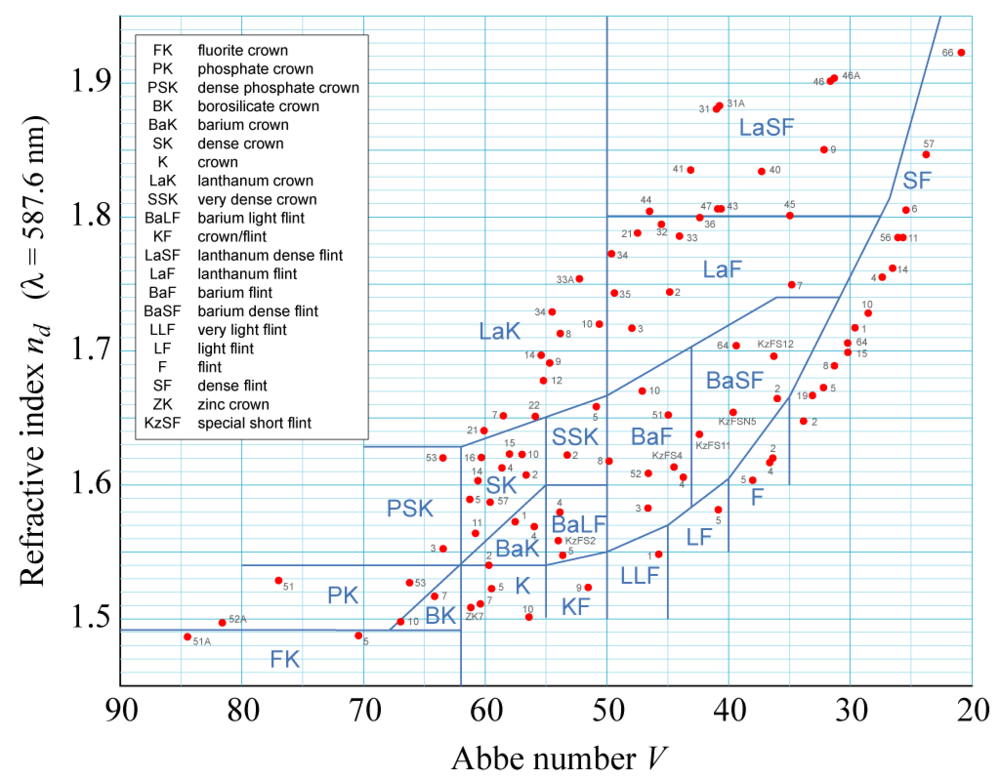
\includegraphics[width=10cm]{figures/abbe-diagram.png}
\caption{Abbe diagram \cite{Opticsforhire}}
\label{fig:abbe}
\end{figure}

\subsubsection{Calculating Focal Lengths of Lens Pair}

The achromatic doublet can be approximated as a linear system:

\begin{equation} \label{eq:achromat-f_eq}
    \frac{1}{f_1} + \frac{1}{f_2} = \frac{1}{f_{eq}}
\end{equation}

where $f_1$ and $f_2$ are the focal lengths of the first and second element respectively and $f_{eq}$ is the effective focal length of the entire system. Furthermore,

\begin{equation}
    \label{eq:abbe-numbers}
    \frac{1}{f_1 V_1} + \frac{1}{f_2 V_2} = 0
\end{equation}

where $V_1$ and $V_2$ are the Abbe numbers for the first and second elements respectively. 

\bigskip

\underline{Note:} A typical Abbe number for crown glass is about 0.016 and a typical Abbe number for flint glass is about 0.028.

\bigskip

Combining (\eqref{eq:achromat-f_eq}) and (\eqref{eq:abbe-numbers}):

\begin{equation}
    \label{eq:f_1}
    f_1 = \frac{V_1-V_2}{V_1}f_{eq}
\end{equation}

\begin{equation}
    \label{eq:f_2}
    f_2 = -\frac{V_1-V_2}{V_2}f_{eq}
\end{equation}

\subsubsection{Calculating Effective Focal Length}

Both (\eqref{eq:f_1}) and (\eqref{eq:f_2}) can be rearranged to derive the effective focal length $f_{eq}$ as a function of either $f_1$ or $f_2$:

\begin{equation}
    f_{eq} = f_1\frac{V_1}{V_1-V_2}
\end{equation}

\begin{equation}
    f_{eq} = -f_2\frac{V_2}{V_1-V_2}
\end{equation}

\subsubsection{Calculating Radius of Curvature}

Assuming symmetric lenses with equal radii of curvature in the front and back surfaces of each lens, the radii of curvature for each lens denoted $R_1$ and $R_2$ can be found using the following:

\begin{equation}
    R_1 = 2f_{eq}\frac{V_1-V_2}{V_1}(n_1-1)
\end{equation}

\begin{equation}
    R_2 = 2f_{eq}\frac{V_2-V_1}{V_2}(n_2-1)
\end{equation}

where $n_1$ and $n_2$ are the refractive indices of the materials.

\subsubsection{First-Order Model: Thin Lenses in Contact} - move to appendix
\todo{Note: these are Shiqi's derivations. Should be ok but would be good to find source.}

The simplest model assumes lenses are thin and in contact.

Definitions:
\begin{itemize}
    \item $f$: Equivalent focal length of the two lenses.
    \item $f_1$: Focal length of first (convex) lens. Positive.
    \item $f_2$: Focal length of second (concave) lens. Negative.
    \item $s_o$: Object distance of doublet. Equal to object distance of first lens.
    \item $s_i$: Image distance of doublet. Equal to image distance of second lens.
    \item $s_{i,1}$: Image distance of first lens. Equal to object distance of second lens.
\end{itemize}

For first (convex) lens:
\begin{equation}
    \frac{1}{f_1} = \frac{1}{s_o} + \frac{1}{s_{i,1}}
\end{equation}

For second (concave) lens:
\begin{equation}
    \frac{1}{f_2} = -\frac{1}{s_{i,1}} + \frac{1}{s_i}
\end{equation}

Together, by \eqref{eq:achromat-f_eq}:
\begin{align}
    \frac{1}{f} &= \frac{1}{f_1} + \frac{1}{f_2} \\
    &= \frac{1}{s_o} + \frac{1}{s_{i,1}} - \frac{1}{s_{i,1}} + \frac{1}{s_i} \\
    &= \frac{1}{s_o} + \frac{1}{s_i}
\end{align}

This is the Gaussian equation for the thin lens (as in \eqref{eq:thin-lens}), from which object and image distances as well as heights follow. We conclude that this simplified first-order model of an achromatic doublet is equivalent to a thin lens (achromatism is second-order). See Section \ref{sec:thin-singlet-model} for equations as well as their derivations for the focuser and collimator cases.

\textit{Note:} if we modelled the doublet as thin lenses with spacing $d$ between them, we would get the following equivalent focal length $f$ \cite{Boundless_undated-to}:
\begin{equation}
    \frac{1}{f} = \frac{1}{f_1} + \frac{1}{f_2} - \frac{d}{f_1 f_2}
\end{equation}
\textit{}

\subsubsection{First-Order Model: Thick Lenses with Spacing}

This can be thought of as a compound thick lens system.

The equivalent focal length of the doublet is given by \cite{Purdue-Lec32, Hecht-optics-6.1}

\begin{equation}
    \frac{1}{f} = \frac{1}{f_1} + \frac{1}{f_2} - \frac{d}{f_1 f_2}
\end{equation}

Where $d$ is the distance between the second principal plane of the first lens and the first principal plane of the second lens, $f_1$ and $f_2$ are the equivalent focal lengths of the first and second lenses, and $f$ is the equivalent focal length of the doublet.

% Then we have object and image distances given by

% \begin{equation}
%     \frac{1}{f} = \frac{1}{s_o} + \frac{1}{s_{i,1}} + \frac{1}{d - s_{i,1}} + \frac{1}{s_i} - d \left( \frac{1}{s_o} + \frac{1}{s_{i,1}} \right) \left(\frac{1}{d - s_{i,1}} + \frac{1}{s_i} \right)
% \end{equation}

% Where $s_o$ is the object distance of the first lens, $s_{i,1}$ is the image distance of the first lens ($d - s_{i,1}$ is the image distance of the second lens), and $s_i$ is the image distance of the second lens.

% \textit{Note:} Since this is less concise, ray tracing matrices may be employed for derivations. See Section \ref{sec:thick-singlet-model} for example setups. In this case, matrices for thick lenses would sandwich a uniform propagation matrix containing the distance between the vertices of the two lenses.

Additionally, the system may be modelled by a single equivalent thick lens whose principal planes are located at \(f d / f_2\) from the first principal plane of the first lens and \(f d / f_1\) from the second principal plane of the second lens \cite{Hecht-optics-6.1}.

Then equations for the thick singlet model apply---see Section \ref{sec:thick-singlet-model}.


\section{Dichroic Bandpass Filter Model} \todo{Eman}
A Dichroic Bandpass Filter uses dielectric layers on glass that transmit a desired range of wavelengths, and reflects the rest. These filters can be categorized into single-cavity and multi-cavity, based on the model. 
\begin{figure}[H]
    \centering
    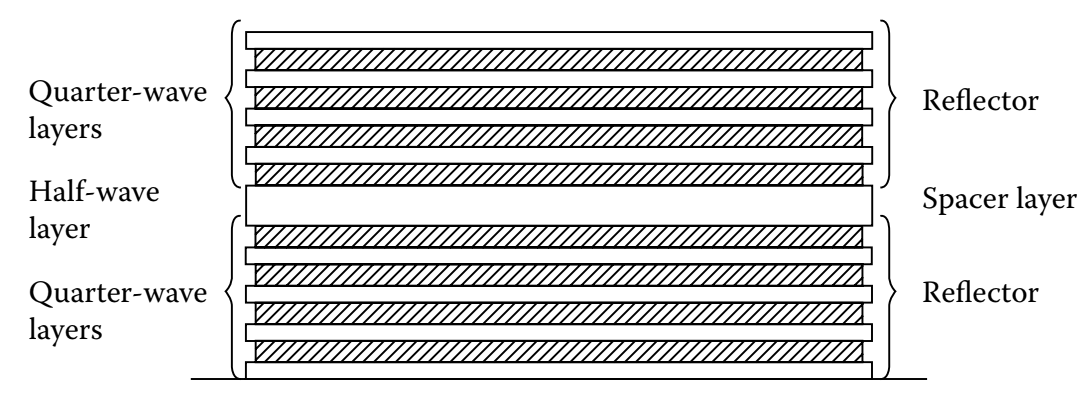
\includegraphics[width=0.7\textwidth]{figures/Single_Layer_Dichroic.png}
    \caption{Single Cavity Dichroic Bandpass Filter}
    \label{fig:my_label}
\end{figure}

\subsection{Phase Shift} - Y
The phase shift of a non-normal incident beam is represented by the following equation:
\\
\begin{equation}
    \lambda_\theta = \lambda_0 \times \sqrt{1 - \left( \frac{n_0}{n^*} \sin\theta \right)^2}
\end{equation}

Where:
\\
$\lambda_\theta$ = the wavelength of the beam at angle of incidence $\theta$
\\
$\lambda_0$ = the wavelength of the beam at normal incident angle
\\
$n_0$ = refractive index of the incident medium 
\\
$n^*$ = effective refractive index of the bandpass filter 
\\\\
Although the filter is made of multiple layers with different indices of refraction, phase shift calculations of the entire system can be done using the effective refractive index, which has a value that is between the highest and lowest indices of the filter layers. 
\\\\
\subsection{Effective Refractive Index}
The effective refractive index is represented by the following equation:
\\
\begin{equation}
    (n^*)^2 = \frac{(0.5A +k\pi)}{\frac{0.5A}{n^2} +2J}
\end{equation}
\\
Where:
\\
$A = (\epsilon_1^0 +\epsilon_2^0 + N\pi)$
\\
A is absorptance ratio; power absorbed by the filter to the power incident on it. 
\\
N = the complex refractive index, $n-ik$
\\
n = refractive index of spacer layer
\\
$k\pi$ = the frequency term, which depends on the type of stack, where $k$ is the propagation constant. 
\\
$J = \frac{\delta_\epsilon}{\delta(\sin^2\phi_e)}$
\\
$\delta = 2\pi n d \cos \theta / \lambda$, where $d$ is the thickness of the spacer layer, and $\theta$ is the angle of incidence of the spacer layer.
\\
There are 3 types of stacks to consider:
\begin{itemize}
    \item Symmetrical, where the beam is incident on the layer with high index.
    \item Asymmetrical, where the beam is incident on the layer with high index.
    \item Asymmetrical, where the beam is incident on the layer with low index.
\end{itemize}

\subsection{Reflected Beam} - Y
According to Cushing, the reflectances from a dichroic bandpass filter is expressed by the following equation:
\begin{equation}
    \sqrt R = \frac{n^* - n_0}{n^* + n_0}
\end{equation}
Where:
\\
$n_0$ = the refractive index of the incident medium
\\
$n^*$ = the effective refractive index of the filter


\subsection{Transmitted Beam}
According to Pidgeon and Smith, the transmittance of the bandpass filter can be expressed by considering the bandpass filter to be comprised of two subsystems, then expressing it through the following equation:

\begin{equation}
T_f = \frac{T_1 T_2}{[1-(R_1R _2)^{1/2}]^2}\frac{1}{1+F\sin^2[\frac{1}{2}(\phi_1\phi_2)-\theta)]}
\end{equation}
\\
Where,
\\
\begin{equation}
    F=\frac{4(R_1R_2)^{1/2}}{[1-(R_1R_2)^{1/2}]^2}
\end{equation} a Fabry-Perot function
\\
and 
\\
$\delta$ is the phase thickness of a coating
\begin{equation}
\delta = \frac{2\pi n d \cos\theta}{\lambda}
\end{equation}
\\
$T_1$, $T_2$ = the transmittances of the first and second subsystems, respectively. 
\\
$R1$ and $R2$ are the reflectances of the first and second subsystem, respectively. \\
$\phi_1$ and $\phi_2$ are the phase differences of the first and second subsystems, respectively. 
\\
$n$ = refractive index
\\
$d$ = layer thickness
\\
$\theta$ = angle of incidence
\\
$\lambda$ = wavelength in free space

The absorbtance of the system should also be taken into account when calculated transmittance. If $R_1 = 1 - T_1$ and $R_2 = 1 - T_2$ and $\frac{T_1T_2}{(1-R_1R_2)^2}$ then the there is complete transmission at the peak of the pass band.

On the other hand, if absorptance is present in the stacks, the maximum transmission would be $T_{max}=\frac{1}{(1+A/T)^2}$ where $A$ is the absorptance of the stack, and $A + R + T = 1$. As the number of layers in a stack is increased, the reflectance and absorbtance also increase, while maximum transmission decreases. 
\\


\section{Diffractor Models}

\subsection{Surface-Relief Grating Model} \todo{Ginny}
Surface relief gratings have been descoped for the payload due to their low diffraction efficiency relative to VPH gratings, but are implemented to form a numerical baseline for performance comparison.

The surface relief model considered is the transmission diffraction grating mode, where the diffracted rays lie on the opposite side of the grating from the incident rays. Each grating groove can be pictured as being a small, slit-shaped source of diffracted light.

\begin{figure}[H]
\centering
\includegraphics[width=\textwidth]{figures/surface-relief-grating-model.pdf}
\caption{The VPH grism model diagram.}
\label{fig:surface-relief-grating-model}
\end{figure}


\subsubsection{Angular distribution of diffracted wavelengths} - Y
Figure \ref{fig:surface-relief-grating-model} visualizes the diffraction of a beam of monochromatic light as it passes through a transmission grating and disperses the light spatially by wavelength $\lambda$, where $\alpha$ is the incident angle, $\beta$ is angle of the diffracted rays exiting the grating, on the opposite side, and $d$ is the groove spacing of the grating. 

The relationships can be expressed by the grating equation:

\begin{equation}
Gm\lambda = \sin\alpha + \sin\beta
\end{equation}

which can be rearranged as:

\begin{equation}
\beta = \arcsin(Gm\lambda - \sin\alpha)
\end{equation}

Where $G = 1/d$ is the groove density of the transmission diffraction grating, and $m$ is the diffraction order (or spectral order). Therefore, to isolate for the angular locations of the principle intensity maxima when light of wavelength $\lambda$ is diffracted from a grating of groove density $G$:

\subsubsection{Angular Dispersion} - Y

Angular dispersion of a grating is a function of the angles of incidence and diffraction, the latter of which is dependent upon groove spacing. Angular dispersion can be increased by increasing the angle of incidence or by decreasing the distance between successive grooves. A grating with a large angular dispersion can produce good resolution in a compact optical system. It is given by:

\begin{equation}
D = \frac{\sin \alpha + \sin \beta}{\lambda \cos\beta}
\end{equation}

\subsubsection{Anamorphic Amplification} - Y
The anamorphic amplificaiton is the ratio $b/a$ of the incident and diffracted beam widths. 

\begin{figure}[H]
\centering
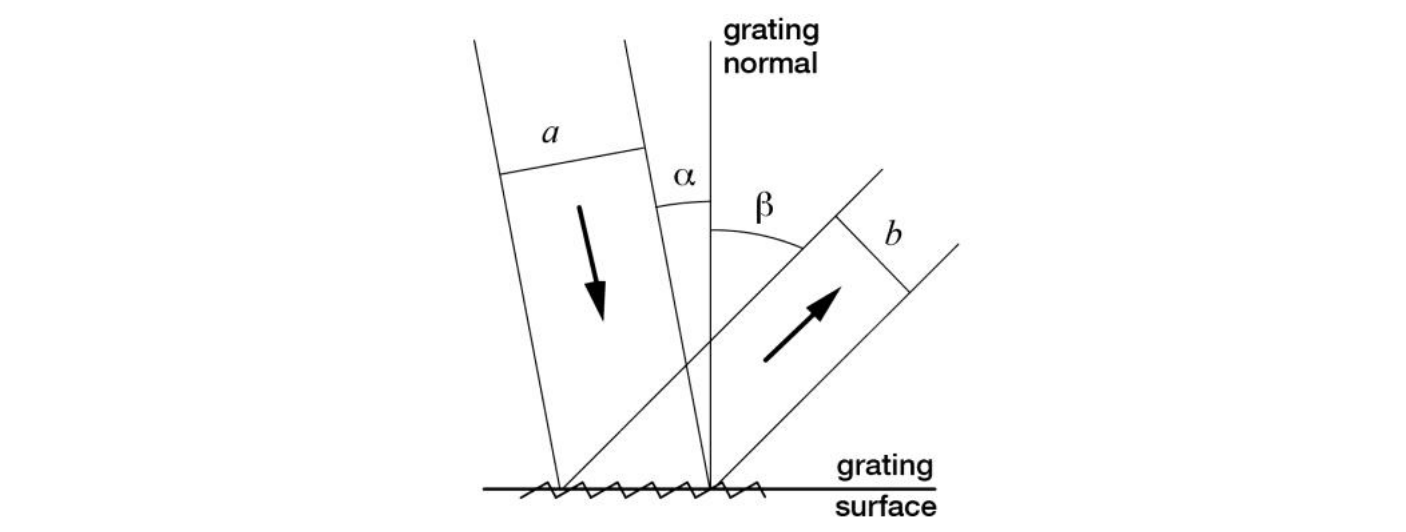
\includegraphics[width=\textwidth]{figures/anamorphic-amplification.png}
\caption{Anamorphic Amplification.}
\label{fig:anamorphic-amplification}
\end{figure}

\begin{equation}
\frac{b}{a} = \frac{\cos\beta}{\cos\alpha}
\end{equation}

\subsubsection{Resolving Power} - Y

The resolving power R of a grating is a measure of its ability to separate adjacent spectral lines of average wavelength $\lambda$. It can be expressed as follows:

\begin{equation}
R = \frac{W(\sin\alpha + \sin\beta)}{\lambda}
\end{equation}

where $W$ is the ruled width of the grating.

The relationship shows that the degree to which the theoretical resolving power is attained depends not only on the angles $\alpha$ and $\beta$, but also the optical quality of the grating surface, the uniformity of the groove spacing, the quality of the associated optics in the system, and the width of the slits. The groove spacing must be kept constant to within about one percent of the wavelength at which theoretical performance is desired. Experimental details, such as slit width, air currents, and vibrations and seriously interfere with the diffraction mechanism. 

\subsection{VPH Grating Model} \todo{Ginny}
A volume phase holographic grating consists of a dichromate gelatin (DCG) film between two glass substrates. It is designed to reduce periodic error that can occur in blazed gratings, and have a high 1st order diffraction peak frequency, low polarization dependence, and uniform performance over broad bandwidths. 

\begin{figure}[H]
\centering
\includegraphics[width=\textwidth]{figures/VPH-grating-model.pdf}
\caption{The VPH grism model diagram.}
\label{fig:VPH-grating-model}
\end{figure}

Figure \ref{fig:VPH-grating-model} shows the geometry and variables of a VPH grating, where $d$ is the film thickness, $n_2$ is the bulk index (average index of refraction between Gragg planes). 

\subsubsection{Angular Distribution of Diffracted Wavelengths} - Y integrate with grism
The light passing through a VPH grating obeys a similar relationship to a surface-relief diffraction grating, given by

\begin{equation}
\frac{m\lambda}{n_i} = \Lambda_g(\sin\alpha_i + \sin\beta_i)
\end{equation}

which can be rearrange to:

\begin{equation}
\beta_i = \arcsin\left(\frac{m\lambda}{n_i\Lambda_g} - \sin\alpha_i \right)
\end{equation}

where $l$ is the wavelength of the light, $n_i$ is the refractive index of the medium with $i$ corresponding to the medium. $\Lambda_g$ is the grating period (the projected separation between the fringes in the plane of the grating, equivalent to the groove spacing in section E.1), $\alpha_i$ is the angle of incidence, and $\beta_i$ is the angle of diffraction from the grating normal. The $\Lambda_g$ shown here is the same as the separation between the fringes of the DCG layer, $\Lambda$. For the general case:

\begin{equation}
\Lambda_g = \frac{\Lambda}{\cos\phi}
\end{equation}

where $\phi$ is the "slant" angle between the grating normal and the plane of the fringes.

\subsubsection{The Bragg Condition} - Y

There exists several condition for high diffraction efficiency. The Bragg condition describes when the light is effectively “reflected” from the plane of the fringes as portrayed by:

\begin{equation}
\beta_2 + \phi = \alpha_2 - \phi
\end{equation}

Combined with the grating equation, the Bragg condition, with the optical index being 1, can be written as:

\begin{equation}
\frac{\lambda}{n_2} = 2\Lambda sin\alpha_{2b}
\end{equation}

where $n_2$ is the refractive index of the DCG layer, and $a_{2b}$ is "Bragg angle", which equals to $\alpha_2 - phi$. 

\subsubsection{First Order Diffraction Efficiencies} - Y
Light nearly obeying the Bragg's Condition condition is still diffracted according to the grating equation, but usually with lower efficiency, and at wavelengths or angles sufficiently
outside the Bragg condition, light passes through the grating
without being diffracted. The Bragg angle is an important parameter for diffraction by VPH gratings as it directly affects efficiency and bandwidth and indirectly affects resolving power.

The diffraction efficiency also depends on the semiamplitude of the refractive-index modulation, $\delta n_2$ and the grating thickness, $d$ in addition to the incidence and diffracted angles. Kogelnik determined first-order diffraction efficiencies at the Bragg condition. For a given refractive-index modulation, Kogelnik’s theory is accurate for Bragg angles above a certain value. For unpolarized light, the Kogelnik efficiency is given by

\begin{equation}
\eta_s = \sin^{2}\left(\frac{\pi \Delta n_2 d}{\lambda cos\alpha_{2b}}\right) + \frac{1}{2} \sin^{2}\left[\frac{\pi \Delta n_2 d}{\lambda cos \alpha_{2b}} \cos(2 \alpha_{2b})\right]
\end{equation}

where the first term is for s-polarized light (the electric vector
is perpendicular to the fringes), and the second term is for p-polarized light (the electric vector is parallel to the fringes).

The figure below shows the relationship between efficiency and grating thickness for two Bragg angles, with fixed $\lambda$ and $n_2$.

\begin{figure}[H]
\centering
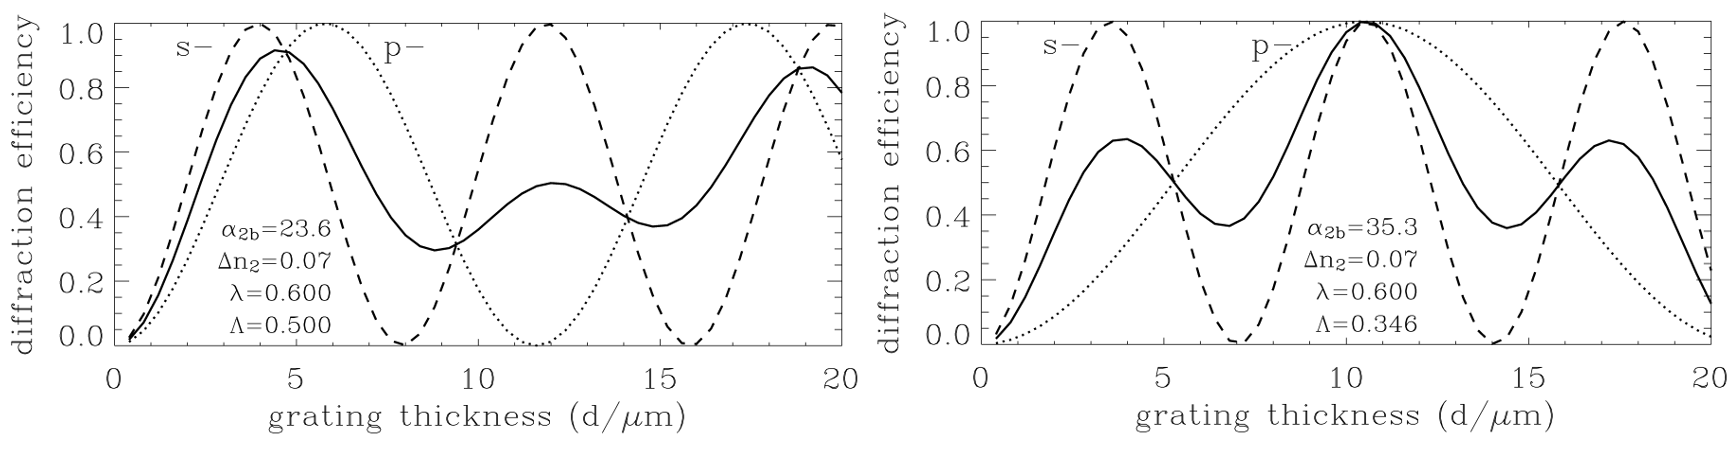
\includegraphics[width=\textwidth]{figures/diffraction-efficiency-to-thickness.png}
\caption{The relationship between diffraction efficiency and grating thickness for two different Bragg angles.}
\label{fig:diffraction-efficiency-to-thickness}
\end{figure}

\subsubsection{Efficiency and Wavelength} - Y
As the wavelength deviates from the Bragg's wavelength, the efficiency decreases by the following approximated formula a for the full width at half-maximum (FWHM) of the efficiency bandwidth ($\Delta \lambda_{eff}$) in first order:

\begin{equation}
\frac{\Delta \lambda_{eff}}{\lambda} \approx \frac{\Lambda}{d} \cot \alpha_{2b}
\end{equation}

This shows that increasing the thickness of the VPH grating decreases the efficiency, also represented in the figure below.

\begin{figure}[H]
\centering
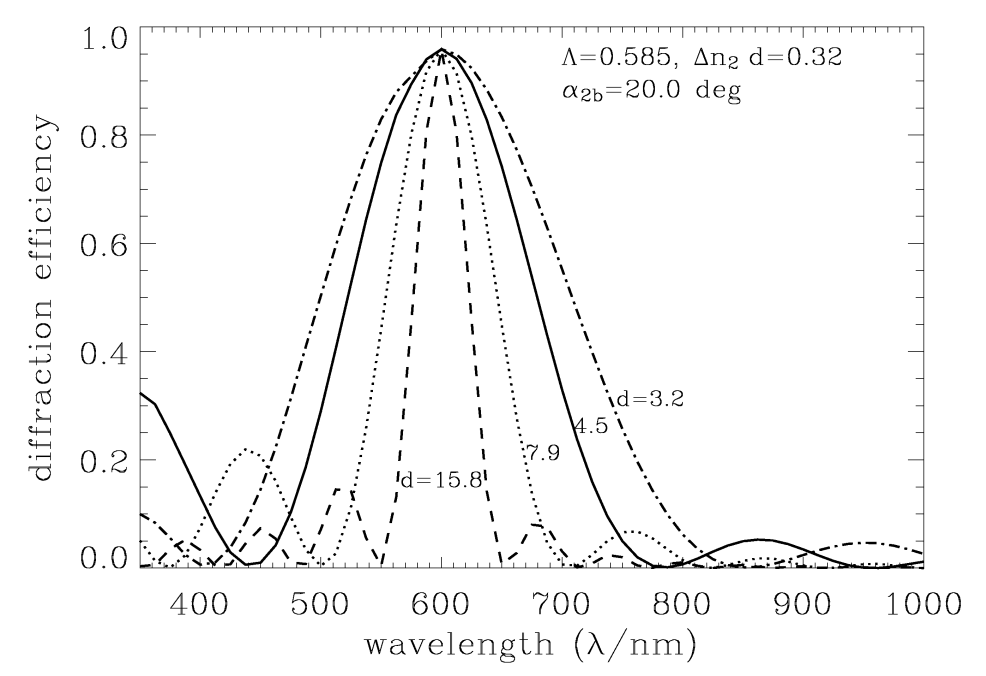
\includegraphics[width=\textwidth]{figures/efficiency-and-wavelength.png}
\caption{The relationship between efficiency and wavelength for four different grating thicknesses.}
\label{fig:efficiency-and-wavelength}
\end{figure}

\subsection{VPH Grism Model} \todo{Kejsi, David}

A grism is a compound optical element composed of a diffraction grating sandwiched between prisms \cite{noauthor_2019-yh}.

\begin{figure}[H]
\centering
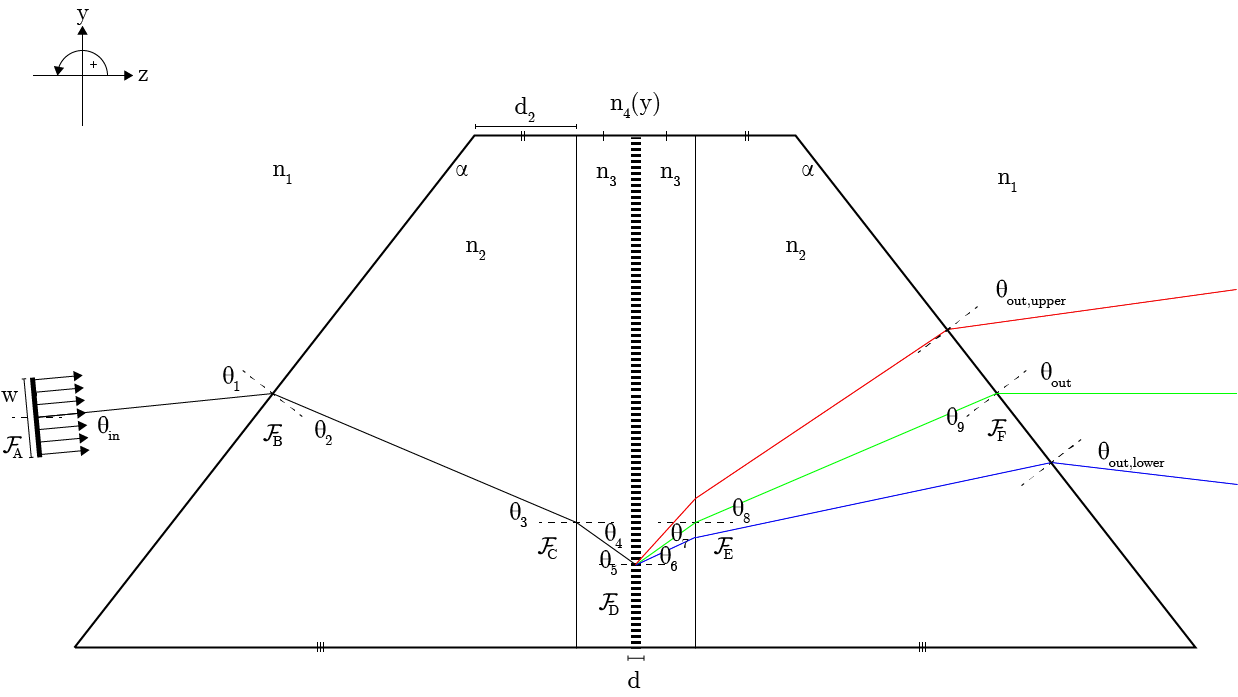
\includegraphics[width=\textwidth]{figures/grism-model.png}
\caption{The VPH grism model diagram.}
\label{fig:grism-model}
\end{figure}

Where $n_1$, $n_2$, and $n_3$ are the indices of refraction of the external medium, prism medium, and VPH hermetic seal medium, respectively. $n_4$ is the sinusoidally-varying index of refraction of the dichromated gelatin material of the VPH grating. 

\subsubsection{Angular distribution of diffracted wavelengths} - Y \todo{David}

An important parameter that defines the performance of a grism is the angular distribution of diffracted wavelengths. This is, in other words, a mapping between the wavelengths produced by the diffractor and the angles those wavelengths leave the component. To solve for this mapping, we observe a bundle of collimated light entering the grism at some angle and successively apply Snell's law at every interface and the diffraction equation at the grating surface. We begin as:

\begin{equation}
\theta_1 = \theta_{in} + \alpha
\end{equation}

Where $\alpha$ is the apex angle of the prisms. In this model, the prisms are assumed to be symmetrical, but they need not be. A symmetrical grism is typically shorter height-wise compared to a non-symmetrical grism \cite{Hill2003-ko}, so is pursued in this design. By Snell's law \cite{Wikipedia_contributors_undated-ti}:

\begin{align} 
n_1 \sin\left( \theta_1 \right) &= n_2 \sin\left( \theta_2 \right) \\ 
\theta_2 &= \arcsin\left( \frac{n_1}{n_2} \sin\left( \theta_1 \right) \right) 
\end{align} 

\begin{equation}
\theta_3 = \alpha - \theta_2
\end{equation}

\begin{equation}
\theta_4 = \arcsin\left( \frac{n_2}{n_3} \sin\left( \theta_3 \right) \right) 
\end{equation}


\begin{equation}
\theta_5 = \theta_4
\end{equation}

A VPH grating diffracts light according to the standard grating equation in the same manner as a classical surface-relief grating, represented by \cite{Barden1999-vq, Barden2000-sv}:
\begin{equation} 
m\nu\lambda = \sin\left( \alpha \right) - \sin\left( \beta \right) \label{eq:grating}
\end{equation} 
where $m$ is the order of diffraction, $\nu$ is the grating frequency, $\lambda$ is the wavelength of light of interest, $\alpha$ is the angle of incidence, and $\beta$ is the angle of diffraction of this wavelength \cite{Barden1999-vq, Barden2000-sv}. Hence:

\begin{align} 
m\nu\lambda &= \sin\left( \theta_5 \right) - \sin\left( \theta_6 \right) \\
\sin\left( \theta_6 \right) &= \sin\left(\theta_5 \right) - m\nu\lambda \\
\theta_6 &= \arcsin\left( \sin\left( \theta_5 \right) - m\nu\lambda \right)
\end{align}

\begin{equation}
\theta_7 = \theta_6
\end{equation}

\begin{equation}
\theta_8 = \arcsin\left( \frac{n_3}{n_2} \sin\left( \theta_7 \right) \right) 
\end{equation}

\begin{equation}
\theta_9 = \theta_8 - \alpha
\end{equation}

\begin{equation}
\theta_{10} = \arcsin\left( \frac{n_2}{n_1} \sin\left( \theta_9 \right) \right)
\end{equation}

Thus,

\begin{equation}
\boxed{\theta_{out} = \theta_{10} + \alpha}
\end{equation}

Assumes:
\begin{itemize}
    \item Angles are small enough or grism is large enough that rays intersect all surfaces of the grism.\footnote{In other words, no light escapes the grism prematurely.}
\end{itemize}

\subsubsection{Undeviated wavelength} - Y \todo{David}
The undeviated wavelength is the wavelength which exits the grating at an angle equal and opposite to the angle of incidence with respect to the grating surface normal, in such a way as:

\begin{equation}
\alpha = -\beta
\end{equation}

Where $\alpha$ is the angle of incidence, and $\beta$ is the angle of diffraction. Equation \eqref{eq:grating} can then be simplified as follows:

\begin{equation}
m\nu\lambda &= \sin\left( \alpha \right) - \sin\left( -\alpha \right)    
\end{equation}

By negative angle identity:

\begin{align}
m\nu\lambda &= 2\sin\left( \alpha \right) \\
\Aboxed{\lambda_g &= 2 \frac{\sin\left( \alpha \right)}{m\nu}} \label{eq:bragg}
\end{align}

Where $\lambda_g$ is the undeviated wavelength. Equation \eqref{eq:bragg} is a simplified form of the Bragg condition, which assumes the grating fringes are normal to the grating surface \cite{Barden2000-sv}.

\subsubsection{Diffraction Efficiency} - Y \todo{Kejsi}
The efficiency of the diffracted energy for a VPH grating is dependent on the undeviated wavelength and incident angle. For a transmission VPH grating with fringe structure normal to the grating surface, the diffraction efficiency for the two planes of polarization can be estimated by using the efficiency equation for a VPH grating and the transmittance of the prism medium. 
\begin{equation}
\eta_s = \sin^{2}\left(\frac{\pi \Delta n_g d}{\lambda cos\alpha_{g}}\right) + \frac{1}{2} \sin^{2}\left[\frac{\pi \Delta n_g d}{\lambda cos \alpha_{g}} \cos(2 \alpha_{g})\right]
\label{eq:energy-diffract}
\end{equation}

Where $\eta_s$ is the diffraction efficiency with respect to the plane of incidence, $\Delta n_g$ is the index modulation contrast, d is the grating thickness and $\alpha_g$ is the angle of incidence \cite{Barden2000-sv}. 
This equation is valid when the following equation is satisfied:
\begin{equation}
Q = \frac{2\pi\lambda d}{n_g \Lambda^2} > 10
\end{equation}
Where $\Lambda$ is $\frac{1}{v_g}$, $v_g$ being the fringe frequency.

Equation \ref{eq:energy-diffract} does not assume the Bragg condition, but the closer the incident angle, $\alpha$ and the undeviated wavelength, $\lambda_g$ are to the Bragg condition, the more efficiently light is diffracted through the grating. 

The diffraction efficiency of the grism can then be found with: 
\begin{equation}
    \eta = \eta_s \cdot T_p \cdot T_p
\end{equation}
Where $T_p$ is the transmittance of the prism medium. 



\subsubsection{Resolvance} - Y merge with grism possibly \todo{Kejsi}

Resolvance or resolving power is a common way of expressing resolution for a grating. Grisms can range from low to high resolving powers, typically in the range of 280 to 8200 \cite{Ebizuka2011-pr}. Diffraction gratings have multiple grooves that follow the same relations as a double slit. The expression for resolving power of a grating is derived by using the intensity expression for a double slit grating. 

\begin{figure}[H]
\centering
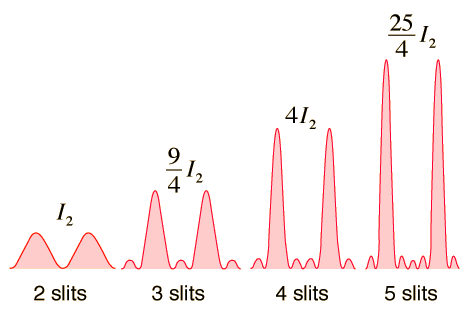
\includegraphics[width=0.5\textwidth]{figures/grating_intensity_curves.png}
\caption{The intensity curves for gratings with varying numbers of slits. Increasing the slits improves the resolution by sharpening the intensity curves.}
\label{fig:grating-intensity}
\end{figure}

The peaks have a phase difference of $\delta$ = 2m$\pi$. The closest minimums occur $\frac{\pi}{2}$ away from the peak, which occurs for a phase change of: 
\begin{equation}
\Delta \delta = \frac{2\pi}{N}
\end{equation}
Where N is the number of slits.

\begin{figure}[H]
\centering
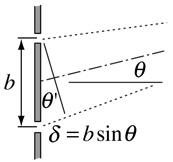
\includegraphics[width=0.5\textwidth]{figures/grating-set-up.png}
\caption{A two-slit grating showing the parameters b, $\theta$, and $\delta$}
\label{fig:grating-set-up}
\end{figure}

From the figure, 
\begin{equation}
\delta = \frac{2\pi}{\lambda}b\sin{\theta}
\end{equation}
The differential of the above is: 
\begin{equation}
d\delta = \frac{2\pi}{\lambda}b\cos{\theta}d\theta
\end{equation}
The maximum condition is:
\begin{equation}
b\sin{\theta} = m\lambda
\end{equation}
With the differential:
\begin{equation}
b\cos{\theta}d\theta = md\lambda
\end{equation}
Substituting both differentials gives:
\begin{equation}
\frac{2\pi}{N} = \frac{2\pi}{\lambda}md\lambda
\end{equation}
This simplifies to the final resolving power formula:
\begin{equation}
\boxed{R = \frac{\lambda}{\Delta \lambda} = mN}
\end{equation}

Where $\lambda$ is the wavelength of interest, $\Delta \lambda$ is the resolution and m is the diffraction order \cite{Hyperphysics}. 





\subsubsection{Diffraction-Limited Spectral Resolution} - Y \todo{Kejsi}
Spectral resolution is the spectral detail in a band, or the width of each band in the dataset. Spectral resolution is inversely proportional to slit width, groove density and diffraction order. The number of slits, N, can be written as  $N = n\cdot w$ where n is the groove density of the grating and w is the slit width.

The expression for spectral resolution can then be written as:
\begin{equation}
\boxed{\Delta \lambda = \frac{\lambda}{m\cdot n\cdot w}}
\end{equation}

\section{Sensor Model}

\begin{table}[H]
\centering
\caption{}
% \label{tab:my-table}
\begin{tabular}{@{}llllll@{}}
\toprule
Parameter          & Symbol                            & Min     & Typical & Max & Unit                                       \\ \midrule
Binning operations & {$n_{\text{bin}}$}                & 1       & -       & -   & -                                          \\
Bit depth          & {$n_{\text{bit}}$}                & 1       & 14      & -   & {\si{\bit}}                                \\
Dark current       & {$i_{\text{dark}}$}               & 0       & -       & -   & {\si{\kilo\electron\per\pixel\per\second}} \\
Integration time   & {$\Delta t$}                      & 0       &         &     & {\si{\milli\second}}                       \\
Mass               & {$M$}                             & 0       & 81      & -   & {\si{\gram}}                               \\
Quantum efficiency & {$\eta_{\text{sensor}}(\lambda)$} & 0       & -       & 1   & -                                          \\
Read noise         & {$\sigma_{\text{read}}$}          & 0       & -       & -   & {\si{\electron}}                           \\
Volume             & {$V$}                             & 0, 0, 0 & -       & -   & {\si{\mm}}                                 \\
Well depth         & {$n_{\text{well}}$}               & 0       & -       & -   & {\si{\kilo\electron}}                      \\ \bottomrule
\end{tabular}
\end{table}

\section{Scrap}

\begin{table}[H]
\centering
\caption{Typical values for grism model parameters \cite{Barden1999-vq}.}
% \label{tab:my-table}
\begin{tabular}{@{}lllll@{}}
\toprule
Parameter        & Min  & Typical & Max  & Unit                  \\ \midrule
{$\eta_2$}       & -    & 1.5     & -    & -                     \\
{$\Delta\eta_2$} & 0.02 & -       & 0.1  & -                     \\
{$d$}            & 4    & -       & 20   & {\si{\micro\m}}       \\
{$\nu$}          & 300  & -       & 6000 & {\si{\L\per\milli\m}} \\ \bottomrule
\end{tabular}
\end{table}



\begin{table}[H]
\centering
\caption{The environmental parameters used to build transmission model A using MODTRAN.}
\label{tab:modtran-A}
\begin{tabular}{@{}ll@{}}
\toprule
Parameters            & Value \\ \midrule
Platform Altitude     &       \\
Geographic Area       &       \\
Ground Type           &       \\
Weather Condition     &       \\
${CO_2}$ Mixing Ratio &       \\
Waveband              &       \\
Solar Altitude Angle  &       \\
Surface Albedo        &       \\ \bottomrule
\end{tabular}
\end{table}
